% Chapter 3

\chapter{Marco teórico}

\label{Chapter3}

%---------------------------------------------------

\section{Estado del arte}

El uso de inteligencia artificial en el sector agroalimentario ha crecido significativamente durante la última década, especialmente en áreas como clasificación de frutas, detección de defectos, estimación de madurez y predicción de vida útil. Este avance ha sido impulsado tanto por el desarrollo de modelos de aprendizaje profundo como por la disponibilidad de sensores ópticos más accesibles. Sin embargo, en cultivos específicos como el dátil Medjool, la aplicación práctica de estas tecnologías sigue siendo limitada.\\

\parencite{kamilaris_deep_2018} realizaron una revisión temprana sobre el uso de redes neuronales y visión por computadora en agricultura, estableciendo las bases para su uso en tareas de clasificación de cultivos y análisis de calidad. Estudios como el de \parencite{garcia_vazquez_scientometric_2021, upadhyay_artificial_2025} han documentado el crecimiento de estas aplicaciones, enfatizando la necesidad de enfoques más integrales y adaptados a entornos reales.\\

En el caso específico de frutas, múltiples autores han demostrado la eficacia de modelos convolucionales para clasificar variedades, predecir estado de madurez o detectar enfermedades superficiales \parencite{rybacki_convolutional_2024, gill_fruit_2023, almomen_date_2023}. Estos algoritmos aprenden directamente de las imágenes y permiten eliminar pasos de preprocesamiento complejos, siempre que cuenten con datasets balanceados y representativos.\\

En paralelo, la espectroscopía de infrarrojo cercano (NIR) ha ganado espacio como técnica no destructiva para estimar características internas de los frutos, como contenido de humedad o azúcares. Estudios como los de \parencite{yuan_determination_2025, wang_improving_2025, chen_prediction_2024} muestran cómo la combinación de NIR con modelos de redes neuronales mejora considerablemente la precisión en predicciones fisicoquímicas.\\

Una tendencia emergente es la integración de distintos tipos de datos en modelos multimodales, como imágenes RGB, espectros NIR y parámetros colorimétricos, lo que ha demostrado ser más robusto frente a variabilidad ambiental y condiciones no controladas \parencite{said_smartripen_2025, passos_deep_2023}. Estos enfoques también permiten predecir variables difíciles de observar a simple vista, como la presencia de hongos o la pérdida de firmeza.\\

Aunque estas técnicas han sido aplicadas exitosamente en frutas como manzana, mango, papaya y jujube, su implementación en Phoenix dactylifera L., y en particular en el dátil Medjool cultivado en México, aún está poco documentada. Algunos trabajos recientes han explorado la clasificación superficial mediante CNNs \parencite{perez-perez_evaluation_2021}, pero la evaluación de características internas sigue siendo un campo abierto, especialmente desde una perspectiva de bajo costo y accesibilidad técnica.\\

En línea con la necesidad de hacer los modelos de aprendizaje profundo más transparentes y confiables, ha surgido un campo conocido como inteligencia artificial explicable (XAI). Técnicas como Grad-CAM, utilizada para visualizar regiones activadas en redes convolucionales aplicadas a imágenes, o SHAP, aplicada a modelos de regresión o clasificación con datos espectrales, permiten interpretar cómo y por qué un modelo toma determinadas decisiones. Estas herramientas no solo ayudan a mejorar la confianza en el sistema, sino que también permiten detectar posibles sesgos o errores estructurales en el entrenamiento \parencite{russel_wavelet_2024, gupta_fruveg-net_2024}.\\

Por lo tanto, existe un área de oportunidad clara para aplicar y adaptar estos avances al caso del dátil Medjool, desarrollando soluciones tecnológicamente viables para productores de la región que necesitan herramientas confiables, no destructivas y económicas.

\newpage

%---------------------------------------------------

\section{Metodología}

Este estudio sigue el enfoque CRISP-DM (Cross-Industry Standard Process for Data Mining), adaptado al contexto agroindustrial y científico del análisis no destructivo del dátil \textit{Medjool}. Esta metodología permite una aproximación flexible, iterativa y centrada en la generación de valor \parencite{shimaoka_evolution_2024, saltz_crisp-dm_2021}.

\begin{figure}[th]
\centering
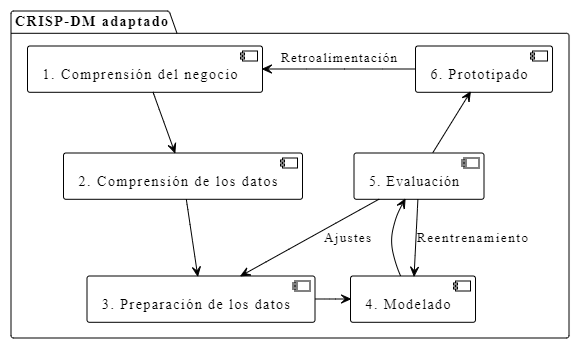
\includegraphics[scale=0.75]{Figures/componentes.png}
\decoRule
\caption[CRISP-DM]{Diagrama de componentes CRISP-DM ajustado a nuestro propósito.}
\label{fig:Componentes_CRISP-DM}
\end{figure}

\subsection{Fase 1: Comprensión del dominio agrícola y científico}

Se analizarán los procesos postcosecha del dátil \textit{Medjool} en el Valle de Mexicali en conjunto con expertos clave del sector:\\

\begin{itemize}
    \item Productores locales con experiencia en recolección y empaque.
    \item El Dr. Juan Pablo García Vázquez (co-director de tesis).
    \item El Dr. Ricardo Salomón Torres (colaborador académico experto en dátil).
\end{itemize}

Este análisis permitirá definir las variables de interés, limitaciones operativas y criterios relevantes.

\subsection{Fase 2: Comprensión y caracterización de los datos}

Se recolectarán muestras representativas de dátil en distintas etapas de madurez y condiciones postcosecha. Cada muestra será sometida a mediciones físico-químicas para establecer etiquetas de referencia:

\begin{table}[h]
\centering
\begin{tabular}{|p{4.5cm}|p{9cm}|}
\hline
\textbf{Variable} & \textbf{Método de medición} \\
\hline

\textbf{Contenido de humedad (\%)} &
Secado en horno con peso constante:
\begin{equation}
\text{Humedad (\%)} = \frac{P_{\text{fresco}} - P_{\text{seco}}}{P_{\text{fresco}}} \times 100
\end{equation}
Alternativas: impedancia dieléctrica, NIR + modelo regresivo. \\
\hline

\textbf{Firmeza (N)} &
Penetrómetro digital o texturómetro. Presión o fuerza aplicada al fruto para determinar su resistencia mecánica. \\
\hline

\textbf{Color (CIELab)} &
Extracción de valores L*, a*, b* mediante espectrofotometría o imagen calibrada. Permite cuantificar brillo y tonalidad. \\
\hline

\textbf{Estado interno (defectos, hongos)} &
Inspección visual tras corte transversal. Validación cualitativa de condiciones internas no visibles externamente. \\
\hline
\end{tabular}
\caption{Variables fisicoquímicas y métodos de medición utilizados en el estudio.}
\label{tab:metodos}
\end{table}

\subsection{Fase 3: Preparación de los datos}

Se desarrollará un protocolo multicanal de adquisición de datos no destructivos con:

\begin{itemize}
    \item Imágenes RGB en condiciones controladas.
    \item Datos espectrales NIR recolectados con sensores portátiles.
    \item Parámetros colorimétricos L*, a*, b*.
    \item Metadatos: fecha, lote, ubicación, condición.
\end{itemize}

Se aplicarán técnicas de preprocesamiento como:

\begin{itemize}
    \item Normalización espectral (e.g., Savitzky-Golay, SNV).
    \item Eliminación de ruido y registros incompletos.
    \item Conversión a formatos estándar tabulares e imagen.
\end{itemize}

\begin{figure}[th]
\centering
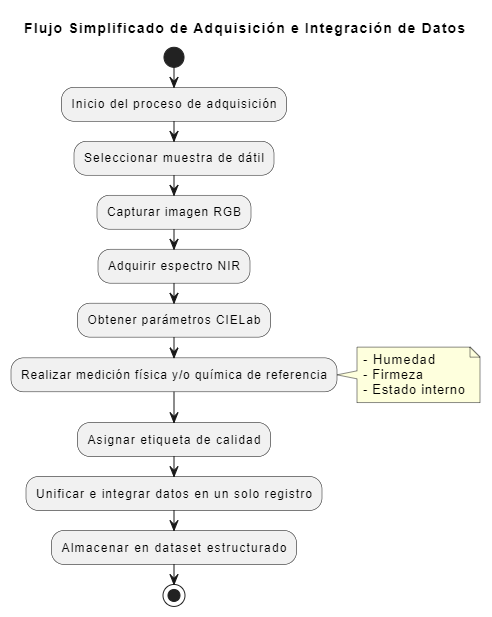
\includegraphics[scale=0.75]{Figures/adquisicion.png}
\decoRule
\caption[Diagrama de adquisicion]{Diagrama de adquisición de variables físico-químicas.}
\label{fig:Diagrama_Adquisicion}
\end{figure}

\subsection{Fase 4: Modelado}

Se entrenarán modelos unimodales y multimodales para tareas de clasificación y regresión. Los modelos incluirán:

\begin{itemize}
    \item CNNs para imágenes RGB.
    \item MLP o CNN-1D para espectros NIR.
    \item Modelos híbridos para fusión de datos.
    \item PLS y Random Forest como modelos de referencia.
\end{itemize}

Para explicar las predicciones se utilizarán técnicas de inteligencia artificial explicable:

\begin{itemize}
    \item \textbf{Grad-CAM}: para mapas de activación en imágenes.
    \item \textbf{SHAP} \parencite{lundberg_unified_2017}: para análisis de variables espectrales y colorimétricas.
\end{itemize}

\subsection{Fase 5: Evaluación}

Se validará el desempeño con métricas según el tipo de tarea:

\begin{itemize}
    \item MAE, RMSE, R\textsuperscript{2} (regresión).
    \item Precisión, sensibilidad, AUC-ROC (clasificación).
    \item Robustez, interpretabilidad y reproducibilidad.
\end{itemize}

\subsection{Fase 6: Implementación del sistema}

El sistema se desarrollará como una solución modular y portable con opciones de despliegue según el entorno:

\begin{itemize}
    \item \textbf{Software especializado} para los diferentes componentes del sistema.
    \item \textbf{Interfaz gráfica} para visualización y control de adquisición.
    \item \textbf{API RESTful} para acceso remoto desde interfaz web o móvil.
    \item \textbf{Jupyter Notebooks}: útil para prototipos, pruebas y visualización interactiva durante las etapas experimentales.
\end{itemize}